\documentclass{article}
\usepackage{graphicx}
\usepackage{enumerate}
\usepackage{booktabs}
\usepackage{geometry}
\usepackage{indentfirst}
\usepackage{mathrsfs}
\usepackage{amssymb}
\usepackage[T1]{fontenc}
\usepackage{mathtools}
\usepackage{amsmath}
\usepackage{amsthm}
\usepackage{babel}
\usepackage{listings}
\usepackage{subfigure}
\usepackage{caption}
\usepackage{pgfplots}
\usepackage{wrapfig}
\usepackage{rotating}
\usepackage[section]{placeins}
\usepackage{subfigure}
\usepackage{textcomp}
\usepackage[normalem]{ulem}
\usepackage{tabularx}
\usepackage{float}
\usepackage{color}
\usepackage{mathrsfs}
\usepackage{setspace}
\begin{document}

\subsection{Whether Mass shootings follow Poisson Distribution}

\subsubsection{Daily Data does not Follow Poisson Distribution}

Using the software we  get the average number of shootings for each day in the week as shown below:

\begin{table} [!htbp]
\begin{center}
\begin{tabular*} {8 cm} {@{\extracolsep{\fill} }cc} 
\toprule
Day & Average Number of Shooting\\
\midrule
Sunday	&	1.73 	\\
Monday	&	0.61	\\
Tuesday	&	0.55  \\
Wednesday&	0.55 	\\
Thursday	&	0.49 	\\
Friday 		&	0.68	\\
Saturday 	& 	1.46 	\\
\bottomrule
\end{tabular*} 
\end{center}
\caption{Average Number of Shooting for Each Day }
\end{table} 

We find that the average number of shootings on weekend is much larger than those on the weekdays. However, if it follows a Poisson distribution, it should be the same for weekend and weekdays. In the following part, we would use Fisher’s null hypothesis testing to reject the idea that it has same probability to have mass shootings on weekday and weekend. Because our data is so big, we can regard it as a normal distribution.


$$H_0:\mu_1=\mu_2$$

\begin{table} [!htbp]
\begin{center}
\begin{tabular*} {14cm} {@{\extracolsep{\fill} }cccc} 
\toprule
Type & Data Number n &Average Number of Shooting $\overline X$ & Standard Deviation $S$\\
\midrule
Weekday	&	1304 & 0.58	& 0.8089\\
Weekend	&	522   &	1.60 & 1.3740\\
\bottomrule
\end{tabular*} 
\end{center}
\caption{Average Number of Shooting for Weekday and Weekend}
\end{table} 

As the variances have a big difference, we would use the pooled T-Test with unequal variances. Apply  Smith-Satterthwaite to get the $\gamma$.

$$\gamma=\frac{(S_1^2/n_1+S_2^2/n_2)^2}{\frac{(S_1/n_1)^2}{n_1-1}+\frac{(S_2/n_2)^2}{n_2-1}}=1247.7$$

we round it down to $\gamma=1247$,so

$$T_\gamma=\frac{(\overline X_1-\overline X_2)-(\mu_1-\mu_2)_0}{\sqrt{S_1^2/n_1+S_2^2/n_2}}=-8.805$$

From the table we get $t_{0.025,300}=1.968$ so we can see $T_\gamma >>t_{0.025,300}>t_{0.025,1247}$ so we can reject $H_0$ at the 0.05 level of significance.

By the Fisher’s null hypothesis testing, we can see the possibility for mass shootings in weekday and weekend is not same, so it would reject the idea that the number of shootings daily follows a Poisson distribution. Because if it follows a Poisson distribution, it would have same probabity to have mass shootings on weekday and weekend



\subsubsection{Whether  Weekly Data Follow Poisson Distribution}


If we consider the data weekly, because the week starts on Sunday,we can get 260 full weeks form the date, we can get the results as below.

\begin{table} [!htbp]
\begin{center}
\begin{tabular*} {14cm} {@{\extracolsep{\fill} }ccc} 
\toprule
Data Number n &Average Number of Shooting $\overline X$ & Standard Deviation $S$\\
\midrule
260 & 6.07	& 5.4448\\
\bottomrule
\end{tabular*} 
\end{center}
\caption{Average Number of Shooting for Each Day }
\end{table} 

If it follows a Poisson distribution, then we should get the result that $\mu=\sigma$, we still use Fisher’s null hypothesis testing here.

$$H_0:\mu=S$$

Here we would use T-test with

$$T_n=\frac{\overline X-\mu}{S/\sqrt n}=1.850$$


From the table we get $t_{0.025,300}=1.968$ so we can see $T_n<t_{0.025,300}<t_{0.025,259}$ so we should not reject $H_0$ at the 0.05 level of significance.

Though we do not reject the $H_0$, we can see the $T_n$ is only slightly smaller than $t_{0.025,300}$ so we would like to discuss further this problem. If we only consider the individual year, we let 52 weeks to become a year and get the following results; (note: here the year is not same as the year we usually discussed)


\begin{table} [!htbp]
\begin{center}
\begin{tabular*} {14cm} {@{\extracolsep{\fill} }cccc} 
\toprule
Year & Data Number n &Average Number of Shooting $\overline X$ & Standard Deviation $S$\\
\midrule
1	&	52 & 4.81	& 2.6645\\
2	&	52   &	5.19 & 2.6423\\
3	&	52 & 6.42	& 3.0828\\
4	&	52   &	7.27  & 3.7632\\
5	&	52 & 6.65	& 2.8414\\
\bottomrule
\end{tabular*} 
\end{center}
\caption{Average Number of Shooting for  Week  by Year}
\end{table} 



If we see it yearly, we would find the standard deviation in each individual year is much smaller than we consider it as a whole. Here we would test the fourth year as an example to see whether it following a Poisson distribution in each individual year.

If it follows a Poisson distribution, then we should get the result that $\mu=\sigma$, we still use Fisher’s null hypothesis testing here.

$$H_0:\mu=S$$

Here we would use T-test with

$$T_n=\frac{\overline X-\mu}{S/\sqrt n}=6.720$$


From the table we get $t_{0.025,50}=2.008$ so we can see $T_n>>t_{0.025,50}>t_{0.025,51}$ so we should  reject $H_0$ at the 0.05 level of significance.

Similarly, we can also reject the idea the number of mass shootings for week follows a Poisson distribution in each individual year.

To conclude, we would say the number of mass shootings for weeks does not follow a Poisson distribution. Though if we see the 5 years together, it would appear to follow, when we see the year separately, the result suggests it does not follow.


\subsubsection{Weather Yearly Data Follow Poisson Distribution}

Then we consider whether the number for year follows the Poisson distribution, we collect the data as follows.

\begin{table} [!htbp]
\begin{center}
\begin{tabular*} {14cm} {@{\extracolsep{\fill} }ccc} 
\toprule
Year & Data Number n & Number of Shooting $ X$ \\
\midrule
2013	&	365 & 252	\\
2014	&	365   &	270 \\
2015	&	365 & 335	\\
2016	&	366   &	382 \\
2016	&	365 & 346	\\
\bottomrule
\end{tabular*} 
\end{center}
\caption{Average Number of Shooting for Each Year }
\end{table} 

By calculation, we get
$$\overline X=317.0\ \ \ \ \ \ \  \ \sigma=2956.00$$


Bacause the data number n=5 is too small, we can't apply the center-limit law. But the huge difference between the $\overline X$ and $\sigma$ suggest that it may not follow a Poisson distribution.

Finally, we would conclude that the number of mass shootings does not follow a Poisson distribution on the large timescale. It may because the shooting is not a random event. People may tend to shoot when they see others shooting. Or it may due to in some month, the economic or social security is not good, it needs further analysis to give a more concrete result.

\section{Weeks with n Shootings}


\subsection{Predicted and Actual Number of Weeks with n Shootings}

By the data above we can draw the actual grapg like below.

\begin{figure}[H]
\begin{center}
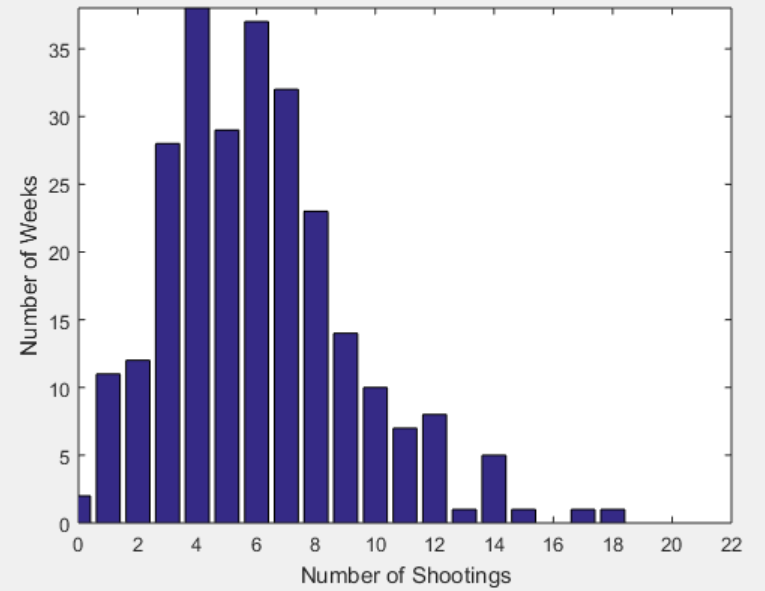
\includegraphics[width=17cm]{actual.png}
\caption{Actual Number of Weeks with n Shootings}
\end{center}
\end{figure}

Though we do not think the number of mass shootings follows the Poisson distribution, since the number is big enough to apply the central limit law, we would use the normal distribution to draw the graph.  We would use $\mu=\overline X=6.07$ and $\sigma=S=5.4448$ then we get the weeks with n mass shootings would be

$$f(n)=\frac{a}{\sqrt{2\pi}}e^{-((n-\mu)/\sigma)^2/2}$$

f(n) would be round up to the nearest integer, then we get the following graph. By testing, we get a=53.8 which allows the sum to be 260.

Then the graph is like below


\begin{figure}[H]
\begin{center}
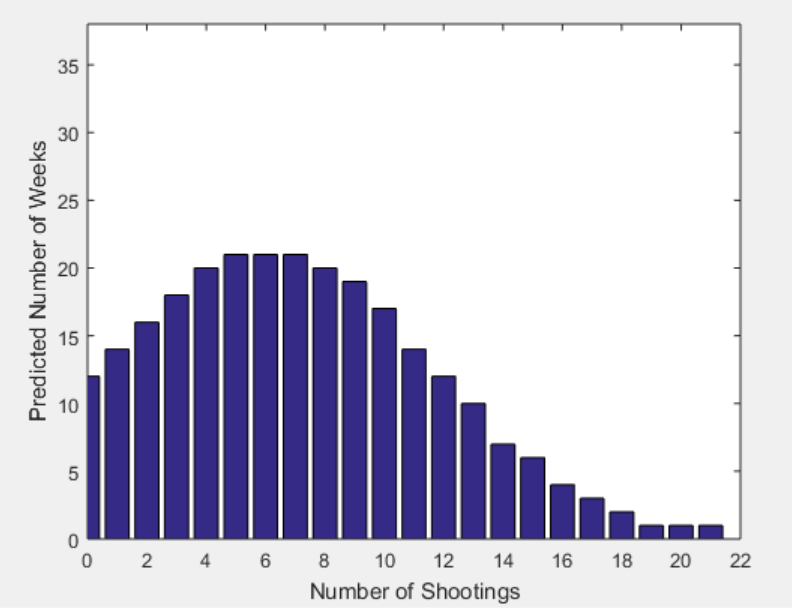
\includegraphics[width=17cm]{Predicted.png}
\caption{Predicted Number of Weeks with n Shootings}
\end{center}
\end{figure}

The big difference with those two picture is caused by the variance. In fact, the variance is much smaller if we consider each year separately, So the actual graph is more steep.





\section{Reference}
%here should have some thing but I believe you have already include it, should I also attatch the matlab and C++ code for the graph?


















\end{document}